%%%%%%%%%%%%%%%%%%%%%%%%%%%%%%%%%%%%%%%%%%%%%%%%%%%%%%%%%%%%%%%%%%%%%%%%%
% ARTICLE ABOUT FATE OF SYNONYMOUS MUTATIONS IN HIV
%%%%%%%%%%%%%%%%%%%%%%%%%%%%%%%%%%%%%%%%%%%%%%%%%%%%%%%%%%%%%%%%%%%%%%%%%
\documentclass[12pt,a4paper,notitlepage,onecolumn]{article}
%%%%%%%%%%%%%%%%%%%%%%%%%%%%%%%%%%%%%%%%%%%%%%%%%%%%%%%%%%%%%%%%%%%%%%%%%
\newcommand{\Author}{Fabio~Zanini and Richard~A.~Neher}
\newcommand{\Title}{(Rise and fall of synonymous mutations)}
\newcommand{\Keywords}{{HIV}, {synonymous}, {population genetics}}
%%%%%%%%%%%%%%%%%%%%%%%%%%%%%%%%%%%%%%%%%%%%%%%%%%%%%%%%%%%%%%%%%%%%%%%%%
\usepackage[english]{babel}
\usepackage[utf8x]{inputenc}
\usepackage{amsmath,amsfonts,amssymb,eucal,eurosym}
\usepackage{color}
\usepackage{subfig}
\usepackage{graphicx}
\usepackage[font=small, format=hang, labelfont={sf,bf}, figurename=Fig.]{caption}
\usepackage{natbib}
\usepackage{pslatex}
\usepackage[colorlinks,linkcolor=red,citecolor=red]{hyperref}
\hypersetup{pdfauthor={\Author}, pdftitle={\Title}, pdfkeywords={\Keywords}}
%%%%%%%%%%%%%%%%%%%%%%%%%%%%%%%%%%%%%%%%%%%%%%%%%%%%%%%%%%%%%%%%%%%%%%%%%
\graphicspath{{./figures/}}
%%%%%%%%%%%%%%%%%%%%%%%%%%%%%%%%%%%%%%%%%%%%%%%%%%%%%%%%%%%%%%%%%%%%%%%%%
%\DeclareMathOperator\de{d\!}
\newcommand{\comment}[1]{\textit{\textcolor{red}{#1}}}
\newcommand{\mut}{\mu}
\newcommand{\mfit}{\langle F\rangle}
\newcommand{\mexpfit}{\langle e^{F}\rangle}
\newcommand{\ox}{r}
\newcommand{\co}{\rho}
\newcommand{\gt}{g}
\newcommand{\locus}{s}
\newcommand{\locuspm}{t}
\newcommand{\OO}{\mathcal{O}}
\newcommand{\env}{\textit{env}}
\newcommand{\rev}{\textit{rev}}
%%%%%%%%%%%%%%%%%%%%%%%%%%%%%%%%%%%%%%%%%%%%%%%%%%%%%%%%%%%%%%%%%%%%%%%%%
\title{\Title}
\author{\Author}
\date{\today}
%%%%%%%%%%%%%%%%%%%%%%%%%%%%%%%%%%%%%%%%%%%%%%%%%%%%%%%%%%%%%%%%%%%%%%%%%
\begin{document}
%%%%%%%%%%%%%%%%%%%%%%%%%%%%%%%%%%%%%%%%%%%%%%%%%%%%%%%%%%%%%%%%%%%%%%%%%
\maketitle

\begin{abstract}
\noindent
Intrapatient HIV evolution is goverened by selection on the protein level in the
arms race with the immune system (killer T-cells and antibodies). Synonymous
mutations do not have an immunity-related phenotype and are often assumed to be
neutral. In this paper, we show that synonymous changes in epitope-rich regions
are often deleterious but still reach frequencies of order one.  We analyze time
series of viral sequences from the V1-C5 part of {\it env} within individual
hosts and observe that synonymous derived alleles rarely fix in the
viral population. Simulations suggest that such synonymous mutations
have a (Malthisuan) selection coefficient of the order of $-0.001$, and that
they are brought up to high frequency by linkage to neighbouring beneficial
nonsynonymous alleles (genetic draft). As far as the biological causes are
concerned, we detect a negative correlation between fixation of an allele and
its involvement in evolutionarily conserved RNA stem-loop structures.
This phenonenon is not observed in other parts of the HIV genome, in which
selective sweeps are less dense and the genetic architecture less constrained.
\end{abstract}

\section{Introduction}

HIV evolves rapidly within a single host during the course of the infection. The
driving forces shaping this process are the high mutation rate and the strong
selection imposed by the host immune system via a wealth of mechanisms, notably
killer T cells (CTLs) and neutralizing
antibodies~\citep{pantaleo_immunopathogenesis_1996}.

In a nutshell, when the host develops a CTL or antibody respose against a
particular viral epitope, rare HIV variants carrying mutated versions of the
epitope, called {\it escape mutants}, acquire a fitness advantage and spread
rapidly in the viral population, within a few months (see
\figurename~\ref{fig:aft}, solid lines). During chronic infection, the
(Malthusian) effect size of this beneficial mutations is of the order of
$0.01$~\citep{neher_recombination_2010}. The viral \env{} gene shows the fastest
rates of adaptation, because is both rich of CTL epitopes and targeted by
antibodies; its sequence diverges at rates of the order of $1\%$ per
year~\citep{shankarappa_consistent_1999}.

Many nucleotide polymorphisms are escape mutations, and in particular are
nonsynonymous, i.e. they appear in protein coding regions and change the amino
acid sequence. Nonetheless, nucleotide changes unrelated to immune escape are
seen, in \env{} and elsewhere, and some of them become abundant alike, often
rapidly. In particular, it is not uncommon for synonymous mutations to reach
frequencies of order one within months from their first appearance (see
\figurename~\ref{fig:aft}, dashed lines). The biological function of these
mutations in the economy of HIV is not well understood. By definition, the
immunological phenotype, which is decided at the protein level, is unaffected,
but other biological and ecological aspects of the viral lifestyle might be
involved. In practice, a couple of RNA-level phenotypes are
known. For example, within \env{} a certain RNA sequence, called \rev{}
response element (RRE), is used by HIV to enhance nuclear export of some of its
transcripts~\citep{fernandes_hiv-1_2012}. Another case is the interaction
between viral reverse transcriptase, viral ssRNA, and the host
tRNA$^\text{Lys3}$: the latter is required for priming viral replication and
bound by a specifical pseudoknotted RNA structure in the viral 5' untranslated
region~\citep{barat_interaction_1991, paillart_vitro_2002}.

Crucially for evolutionary studies, the minor phenotypes caused by synonymous
mutations might have an effect on viral fitness. For instance, recent studies
have shown that genetically engineered HIV strains with skewed codon usage bias
(CUB) patterns towards more or less abundant tRNAs replicate better or worse,
respectively~\citep{ngumbela_quantitative_2008, li_codon-usage-based_2012}.
In this study, we try to characterize the fitness effects of synonymous
polymorphisms that, at some point during the infection, become abundant in the
viral population.

One simple way to assess the neutrality of synonymous mutations is to look at
their level of conservation. Deleterious mutations at functional sites are
expected to be absent or rare across the viral population; vice versa, mutant
alleles that reach high frequencies are expected to be neutral. Confirmatorily,
population genetics shows that the equilibrium frequency of a deleterious allele
with fitness $-s$ is $\mut / |s|$, where $\mut$ is the mutation rate per site
per generation; neutral alleles have no equilibrium frequency and can slowly fix
via genetic drift~\citep{ewens_mathematical_2004}. This approach, albeit
intuitive, works only under the assumption of independent sites. If the focal
synonymous mutant is linked to another, nonneutral allele, its frequency is the
result of the combined fitness effects of both sites. Since recombination in HIV
is known to be rather rare~\citep{neher_recombination_2010,
batorsky_estimate_2011}, the genetic context of the synonymous change at hand
must be taken into account.


\section{Results}
We start from time series of viral nucleotide sequences from single patients,
which span several years of chronic
infection~\citep{shankarappa_consistent_1999, bunnik_autologous_2008,
liu_selection_2006}. Plotting the allele frequencies against time for all
polymorphic sites, it is evident that, although nonsynonymous changes are
widespread, synonymous ones are also present in various occasions at high
frequency (see \figurename~\ref{fig:aft}).
\begin{figure}
\begin{center}
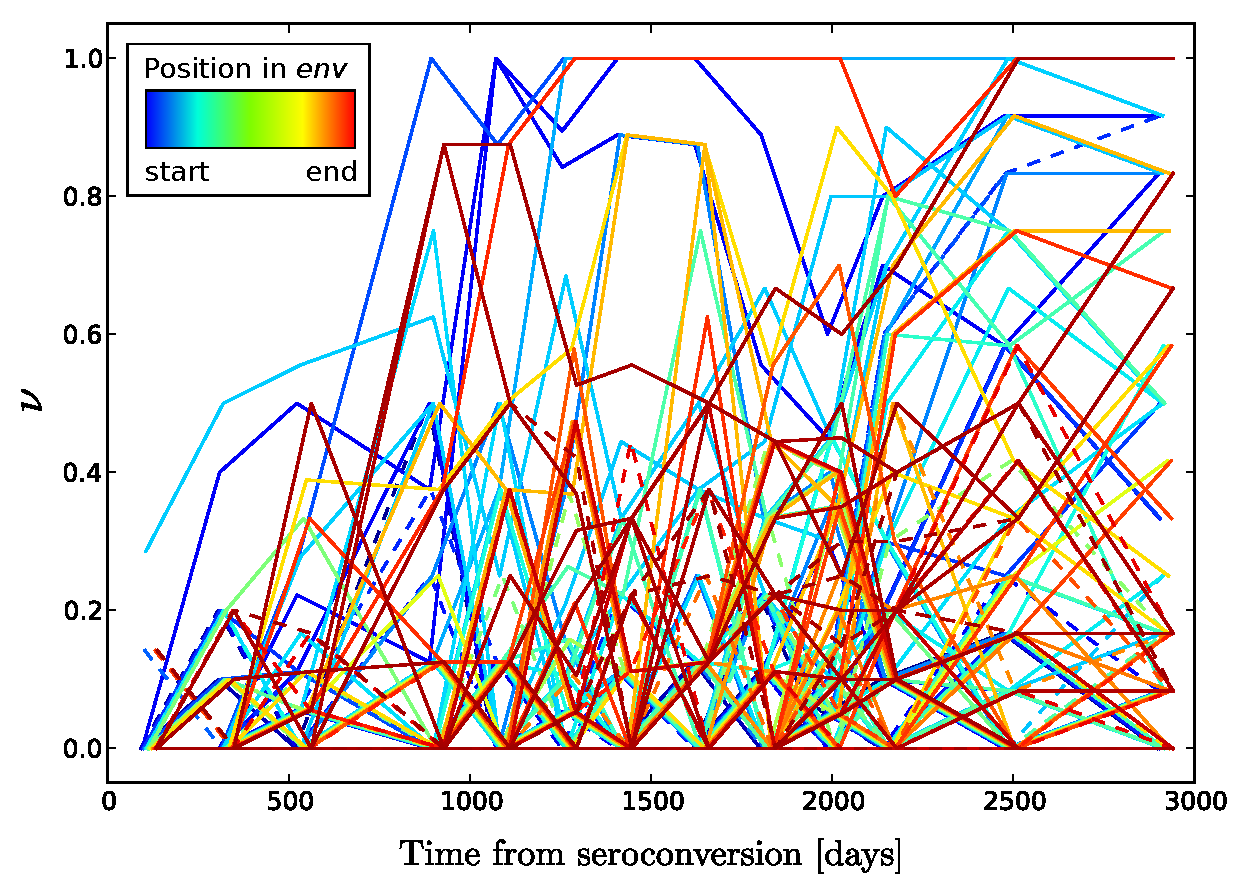
\includegraphics[width=\linewidth]{Shankarappa_allele_freqs_trajectories_syn_nonsynp8}
\caption{Allele frequency trajectories of typical patient, C3-V5, nonsynonymous
(solid) and synonymous mutations (dashed lines). Most synonymous mutations are
not fixed. Colors are set according to the position of the site along the C3-V5
region (red to blue). Data from Ref.~\cite{shankarappa_consistent_1999}.}
\label{fig:aft}
\end{center}
\end{figure}


\begin{figure}
\begin{center}
\subfloat{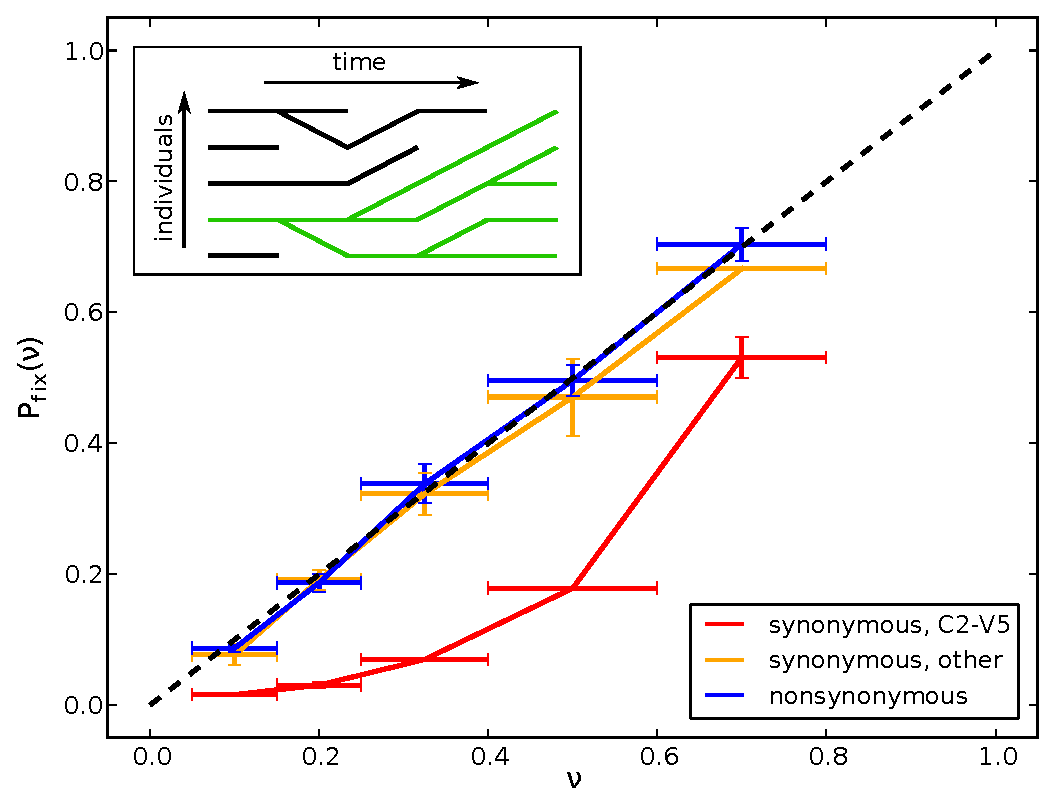
\includegraphics[width=0.49\linewidth]{Bunnik2008_fixmid_syn_ShankanonShanka}}
\subfloat{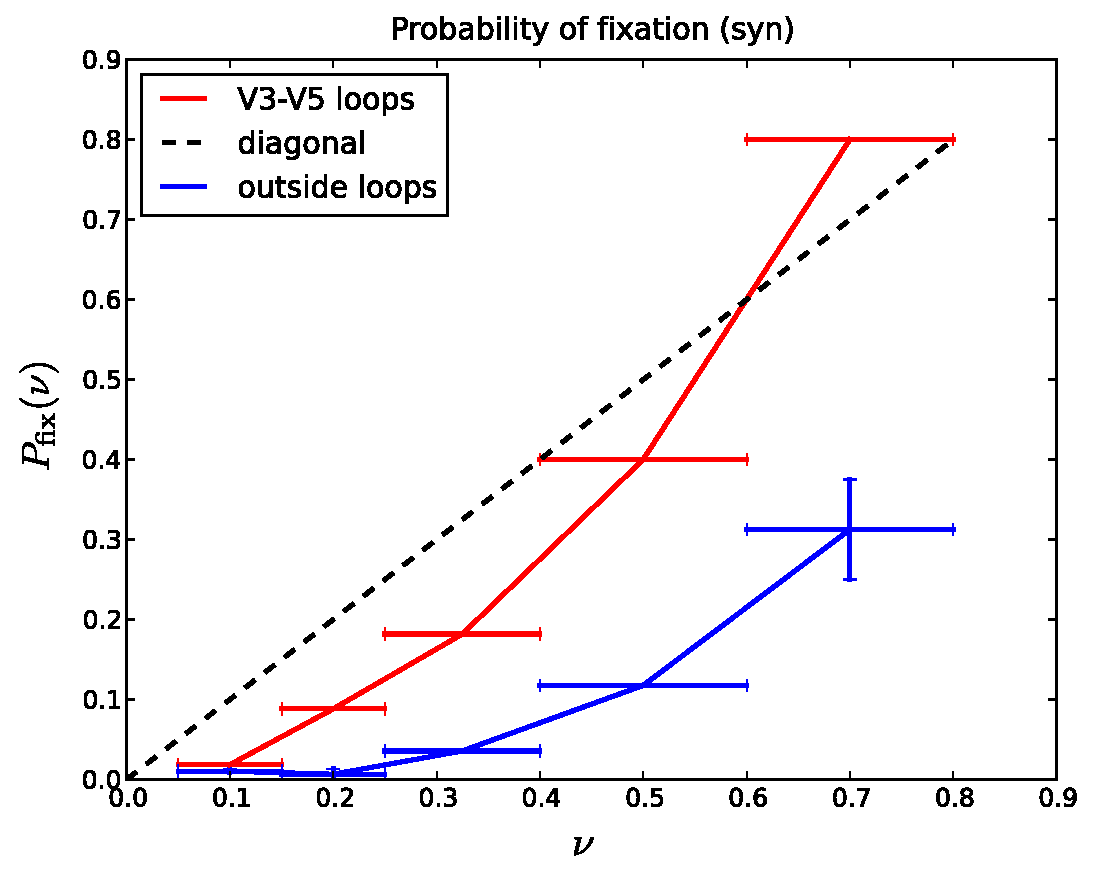
\includegraphics[width=0.49\linewidth]{Shankarappa_fixmid_syn_V_regions}}
\caption{Fixation probability of derived synonymous alleles is strongly
suppressed in C3-V5 versus other parts of the {\it env} gene (left panel).
Especially hard is fixation of new alleles in conserved regions flanking the V
loops (right panel). The black dashed line is the prediction from neutral
theory, for comparison purposes. Data from
Refs.~\cite{shankarappa_consistent_1999, bunnik_autologous_2008}.}
\end{center}
\end{figure}


\begin{figure}
\begin{center}
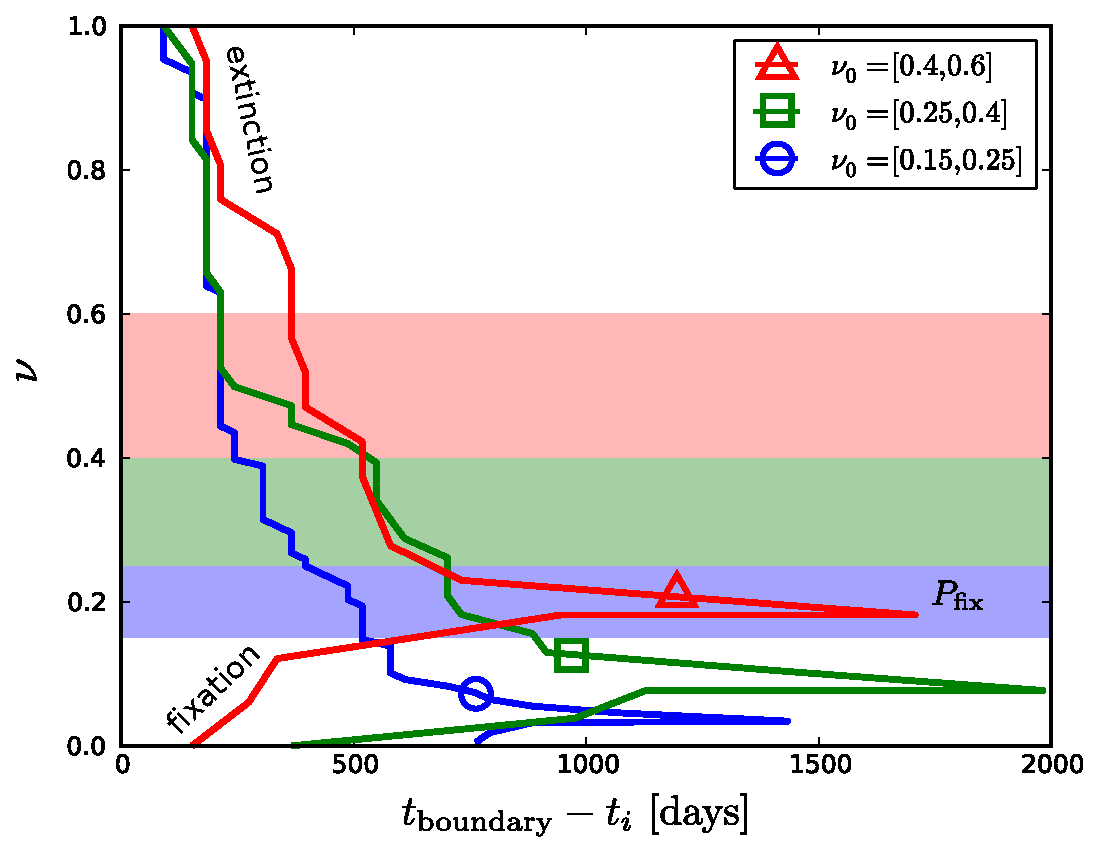
\includegraphics[width=\linewidth]{Shankarappa_fix_loss_dt_times}
\caption{Fixation or extinction times for synonymous alleles starting from
intermediate frequencies. The colored bands are the final fixation probabilities
expected from neutral theory; the observed alleles are fixed less frequently
than expected. The timescale of fixation/extinction is approximately 500 days,
corresponding to a selective effect of $\sim -0.001$.}
\label{fig:fixtimes}
\end{center}
\end{figure}

\begin{figure}
\begin{center}
\subfloat{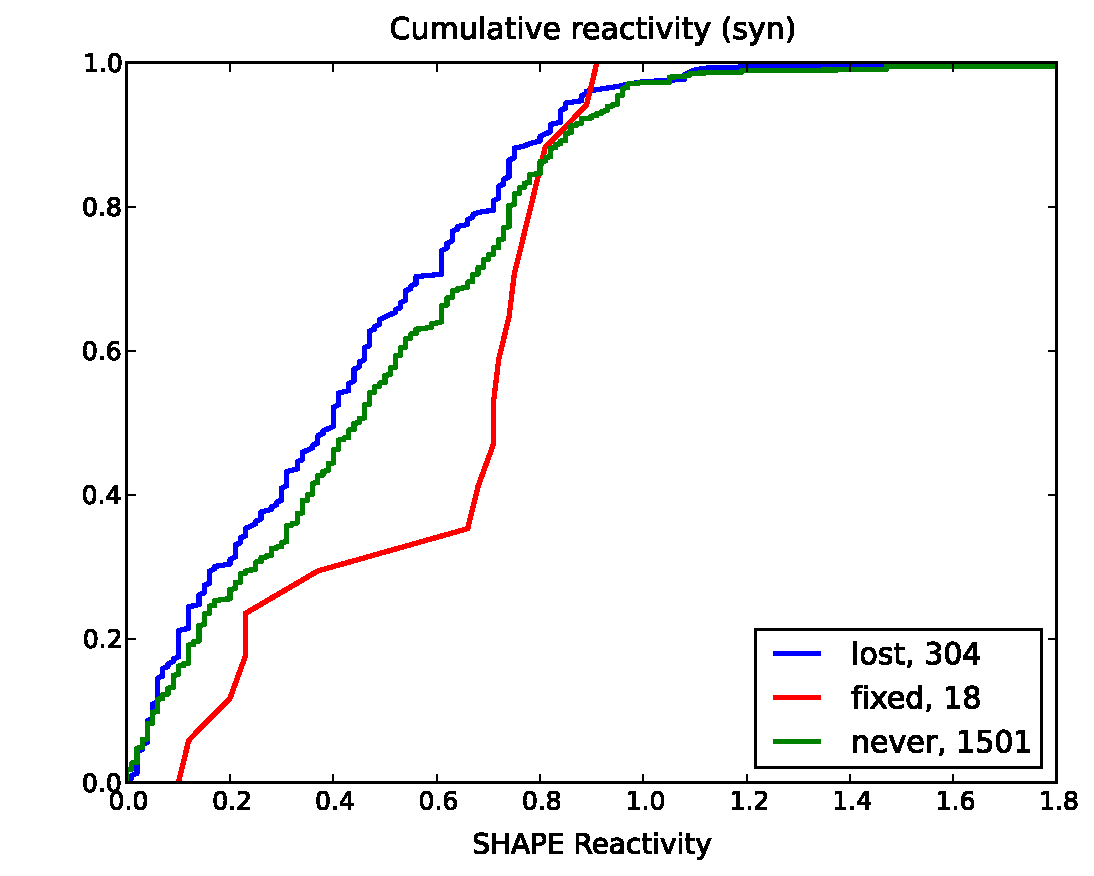
\includegraphics[width=0.49\linewidth]{mixed_Shankarappa_Bunnik2008_Liu_fixation_reactivity_Vandflanking_fromSHAPE}}
\subfloat{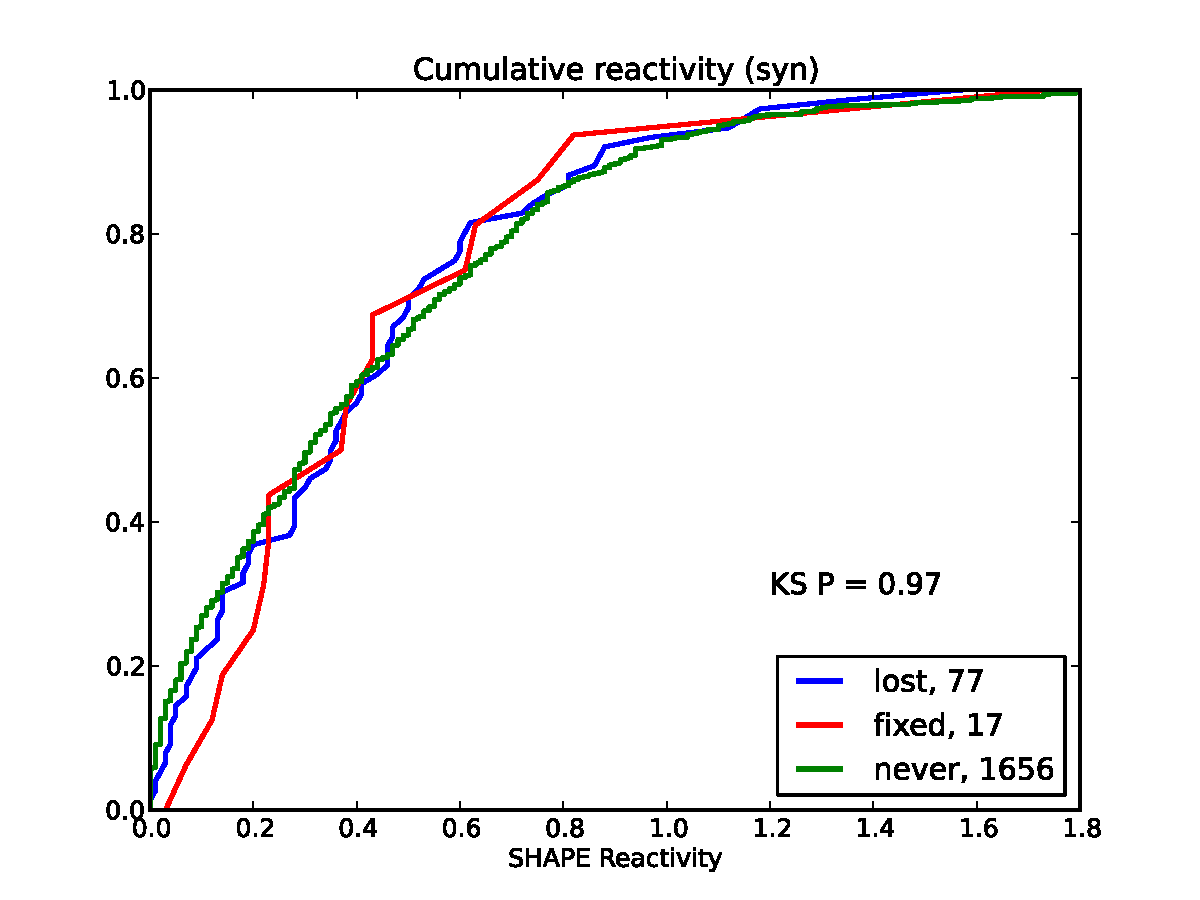
\includegraphics[width=0.49\linewidth]{mixed_Shankarappa_Bunnik2008_Liu_fixation_reactivity_nonVandflanking}}
\caption{Watts et al. have measured the reactivity of HIV nucleotides to {\it in
vitro} chemical attack and shown that some nucleotides are more likely to be
involved in RNA secondary folds. C1-C5 regions, in particular, show conserved
stem-loop structures~\citep{watts_architecture_2009}. We show that among all
derived alleles in those regions reaching frequencies of order one, there is a negative
correlation between fixation and involvement in a base pairing in a RNA stem
(left panel). The rest of the genome does not show any correlation (right
panel). There might be too few silent polymorphisms in the first place, or the
signal might be masked by a lot of non-functional RNA structures. Data from
Refs.~\cite{shankarappa_consistent_1999, bunnik_autologous_2008,
liu_selection_2006}.}
\end{center}
\end{figure}

%\begin{figure}
%\begin{center}
%\subfloat{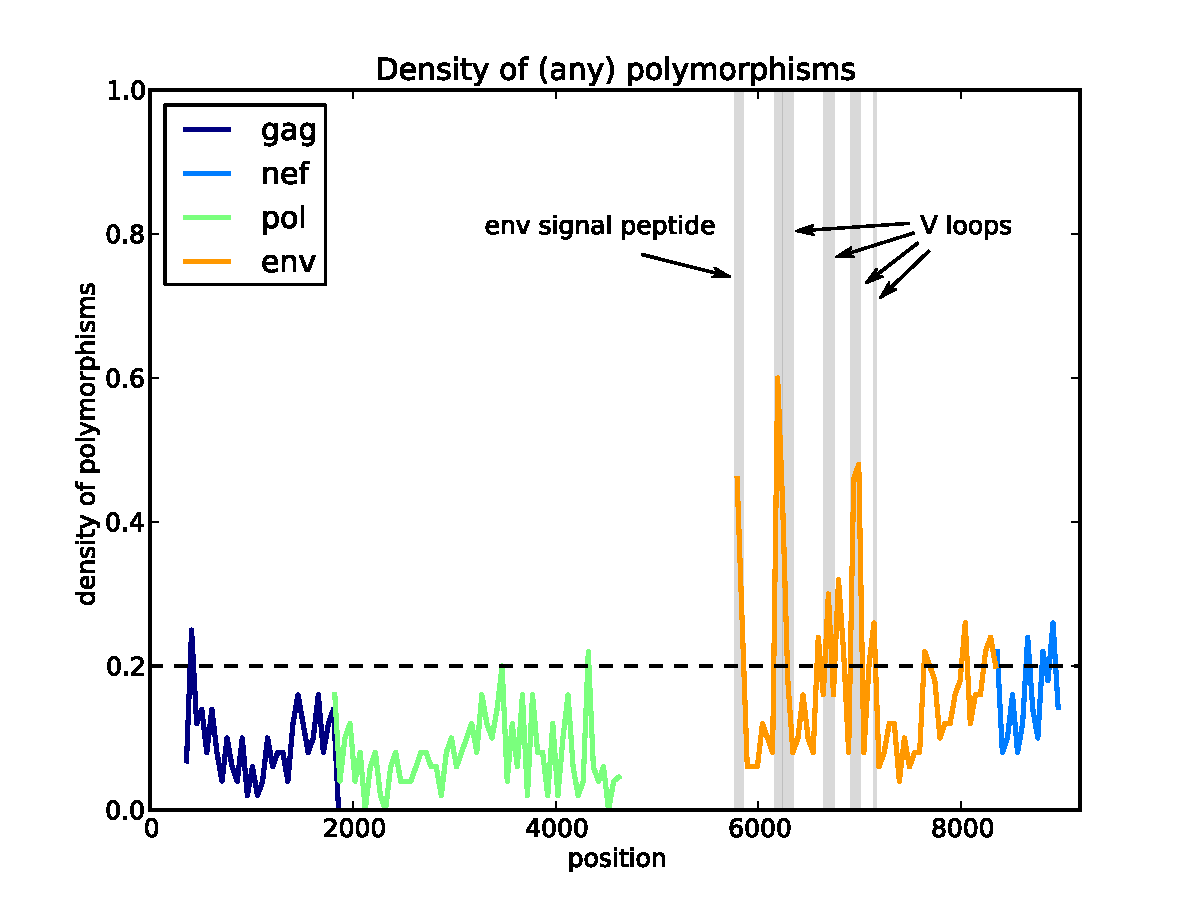
\includegraphics[width=0.49\linewidth]{Henn_density_polymorphisms}}
%\subfloat{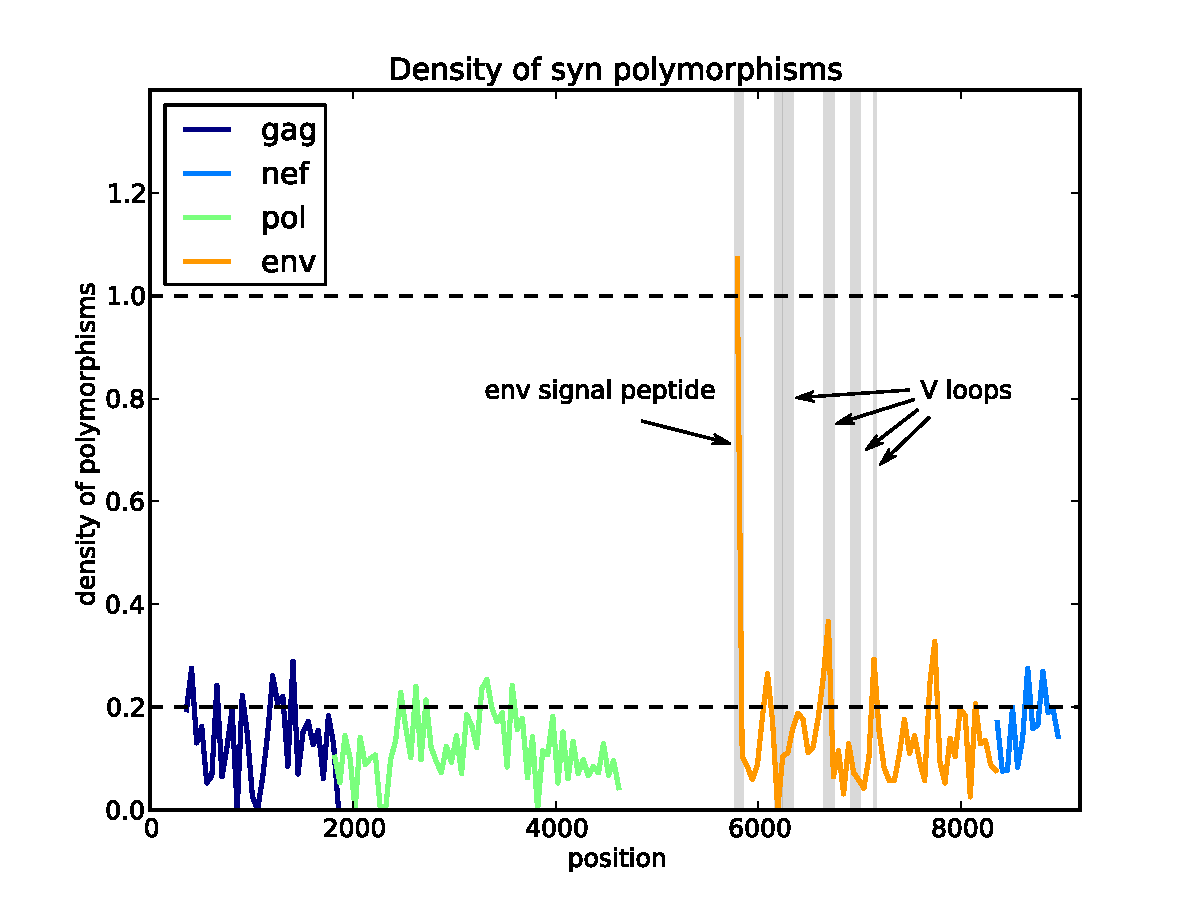
\includegraphics[width=0.49\linewidth]{Henn_density_polymorphisms_syn_over_chances}}
%\caption{The total density of polymorphisms (mostly nonsynonymous ones) is
%highest in the V regions (left panel). The density of synonymous mutations only,
%however, is not enriched there (right panel). This could be due to a more
%deleterious effect of synonymous mutations.}
%\end{center}
%\end{figure}

\begin{figure}
\begin{center}
\subfloat{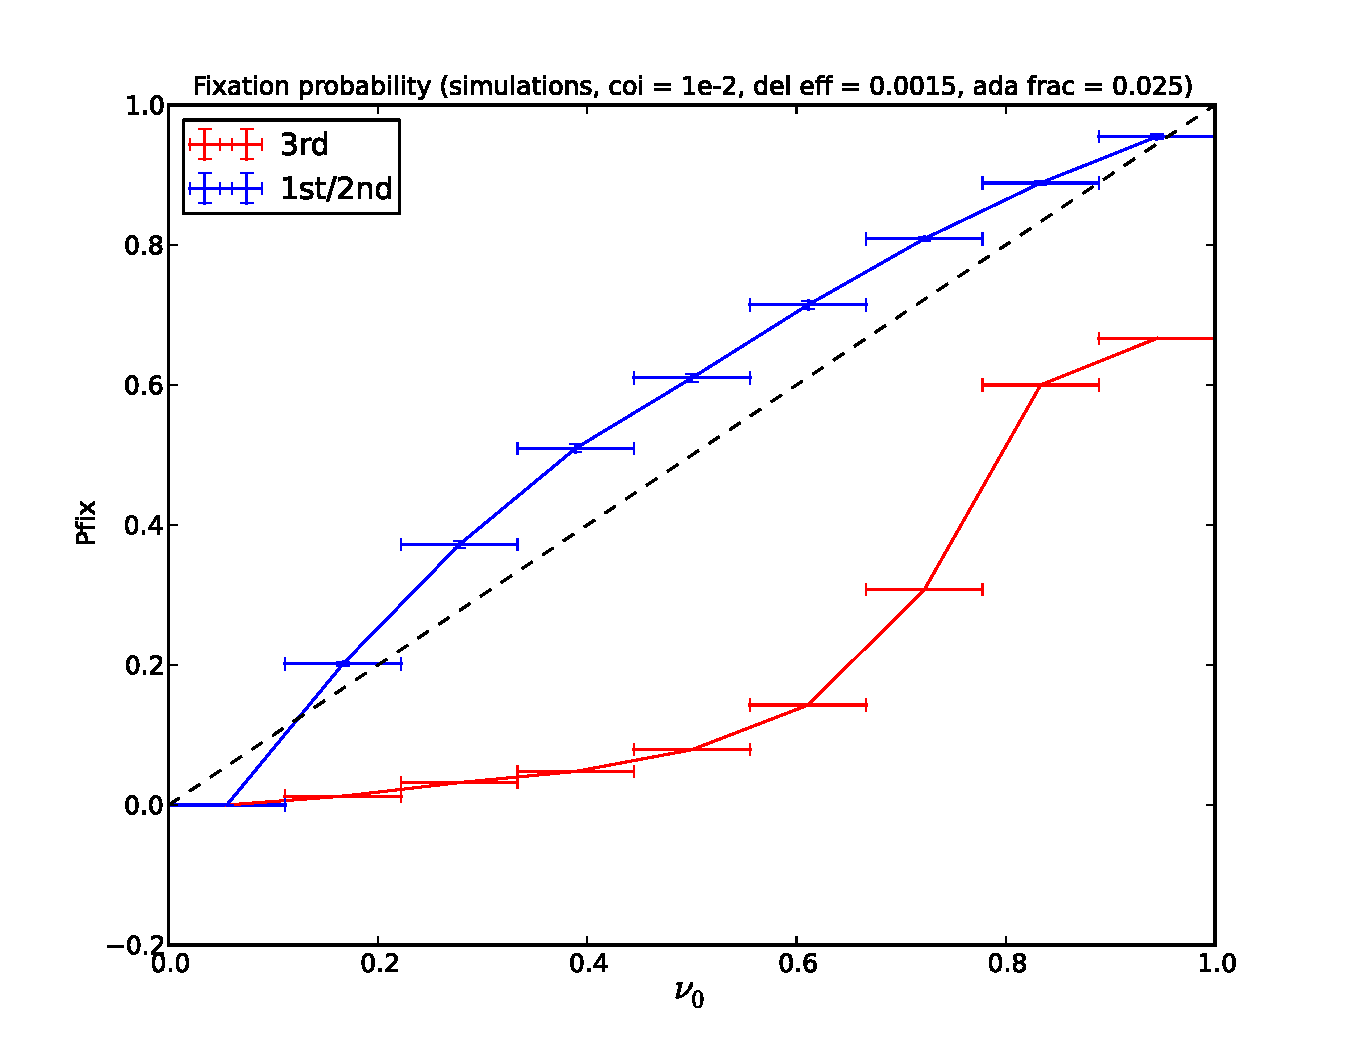
\includegraphics[width=0.49\linewidth]{fixation_probability_shortgenome_N_1e4_epitopes_example_longer}}
\subfloat{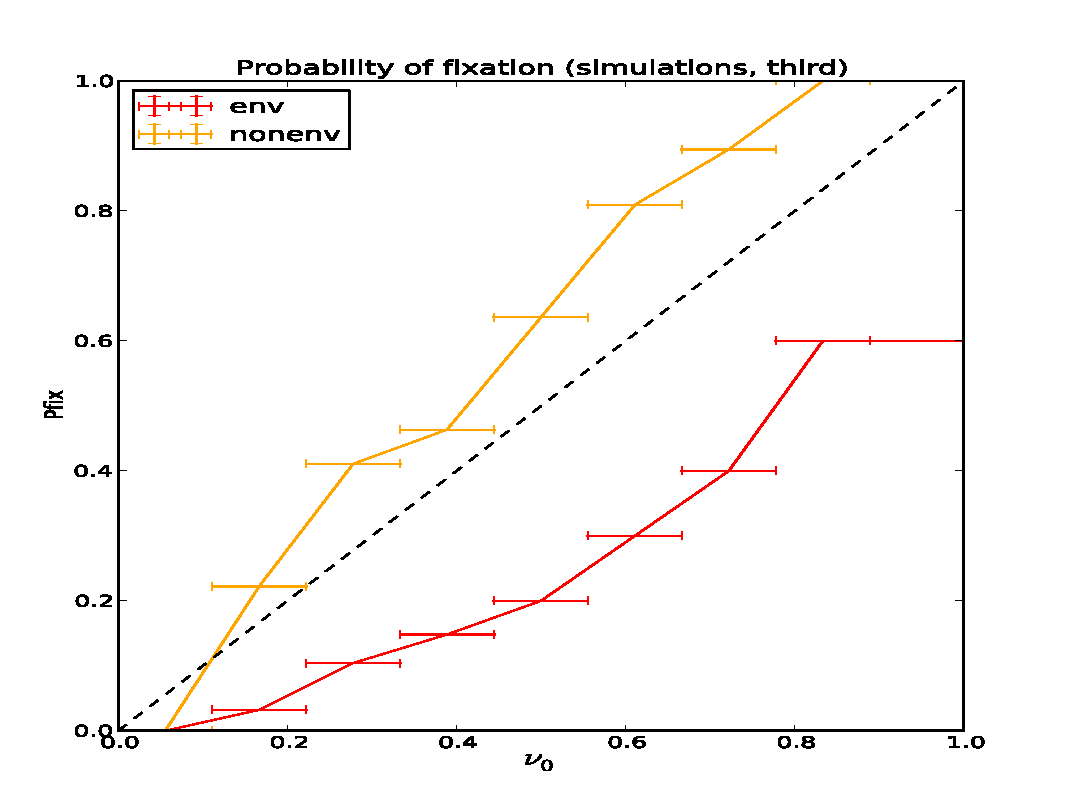
\includegraphics[width=0.49\linewidth]{fixation_probability_N_1e4_3ingredients_3rddel_envnonenv_stopall}}
\caption{Simulations show that the suppression of fixation probability can be
generated by linkage to sweeping nonsynonymous alleles nearby. Two possible
scenarios are competition between escape mutants (left panel) and time-dependent
selection due to immune sytem recognition (right panel).}
\end{center}
\end{figure}

\begin{figure}
\begin{center}
\subfloat{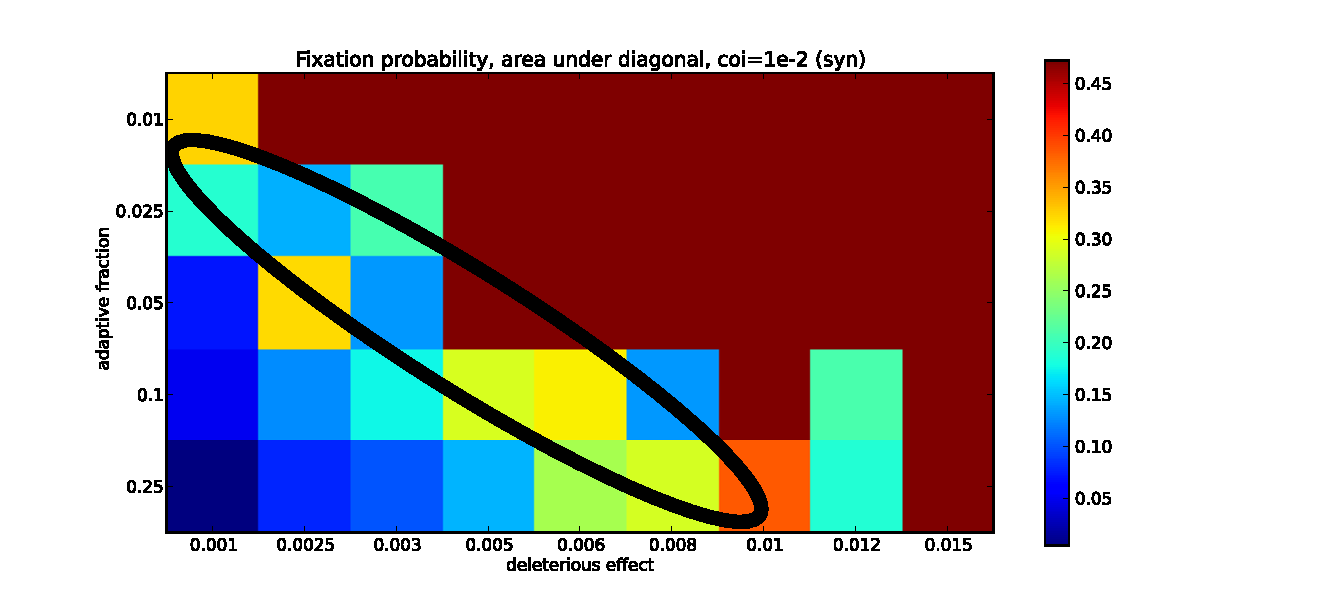
\includegraphics[width=0.49\linewidth]{fixation_loss_shortgenome_area_ada_frac_del_eff_coi_0_01_nescepi_6_heat.pdf}}
\subfloat{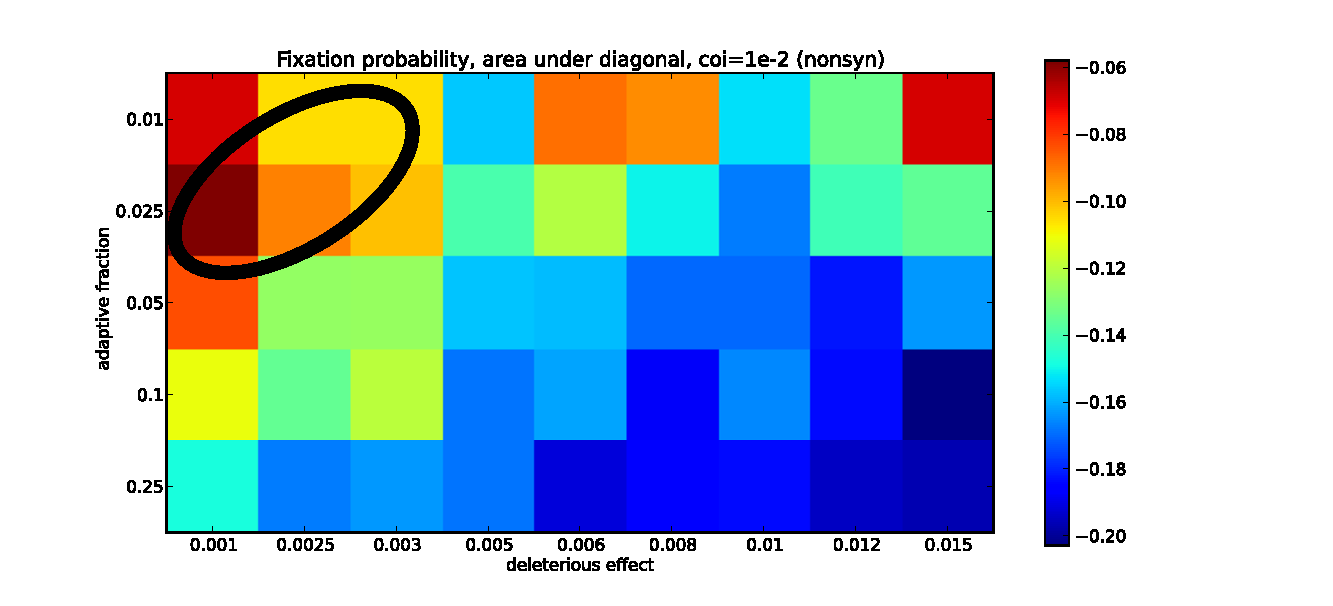
\includegraphics[width=0.49\linewidth]{fixation_loss_shortgenome_area_ada_frac_del_eff_coi_0_01_nescepi_6_nonsyn_heat.pdf}}

\caption{Simulations on the escape competition scenario show that the density of
 selective sweeps and the size of the deleterious effects of synonymous
 mutations are the main driving forces of the phenomenon. A convex fixation
 probability is recovered, as seen in the data, along the diagonal (left panel):
 more dense sweeps can support more deleterious linked mutations. The density of
 sweeps is limited, however, by the nonsynonymous fixation probability, which is
 quite close to neutrality (right panel). Moreover, strong competition between
 escape mutants is required, so that several escape mutants are ``found'' by HIV
within a few months of antibody production.}

\end{center}
\end{figure}

\section{Discussion}
\section{Methods}
\section*{Acknowledgements}

%%%%%%%%%%%%%%%%%%%%%%%%%%%%%%%%%%%%%%%%%%%%%%%%%%%%%%%%%%%%%%%%%%%%%%%%%
\bibliographystyle{natbib}
\bibliography{bib}
%%%%%%%%%%%%%%%%%%%%%%%%%%%%%%%%%%%%%%%%%%%%%%%%%%%%%%%%%%%%%%%%%%%%%%%%%
\end{document}
%%%%%%%%%%%%%%%%%%%%%%%%%%%%%%%%%%%%%%%%%%%%%%%%%%%%%%%%%%%%%%%%%%%%%%%%%

